

\documentclass[12pt, a4paper]{ article}
\usepackage{graphicx}
\setlength{\topmargin}{0in}
\setlength{\headheight}{0in}
\setlength{\headsep}{0in}
\setlength{\textheight}{9.5in}
\setlength{\textwidth}{6.5in}
\setlength{\oddsidemargin}{0in}
\setlength{\evensidemargin}{0in}


\date{}
\begin{document} 
\title{Blinky Lights} 
\author{Kevin Yeap, Steven Morad, Connie Yu, Reid Anetsberger}
\maketitle 

% for comments use. 
% use this style for block comments
\iffalse
    This is a block comment.
    This line is also inside the block comment.
\fi



%PAGE 1===========================================================================================
\noindent
\textbf{Hardware:} 

\vspace{1cm}

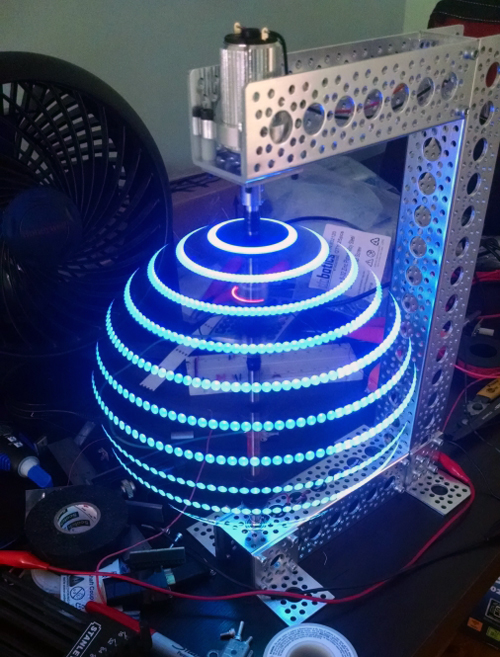
\includegraphics[]{C:/Users/KevinD/Desktop/user_doc/b.PNG}


\vspace {1cm }
\noindent
1. Make sure no objects are obstructing the path of the LED strip. When the hardware is running the LED strip will be rotating at high speeds,  anything obstructing its path must be removed.\\\\
2. Plug in the AC adapter into a wall socket and the other end into the hardware.
\\\\
3. Turn on the hardware by flipping the power switch.
\\\\


WARNINGS: hardware spins at high speeds. Do not attempt to touch the hardware when it is spinning. 
Keep out of reach of children under 6 years of age. If you accidentally swallow hardware, seek professional help or contact a poison control center immediately.


\vspace{6cm}




 %PAGE 1===========================================================================================
\textbf{Bluetooth:} 
1. Turn on bluetooth on your pc and scan for surrounding devices.
 \\\\
2. Connect to the device called "BLINKY LIGHTS"
\\\\
3. Once your pc is connected to "BLINKY LIGHTS", open the software.
\\\\




\indent


\includegraphics[]{C:/Users/KevinD/Documents/GitHub/blinkylights/doc/user_doc/bluetooth.PNG}


\vspace{10cm}







\indent

\textbf{2. Software:} Execute the program . You should be greeted with the following GUI 

\indent

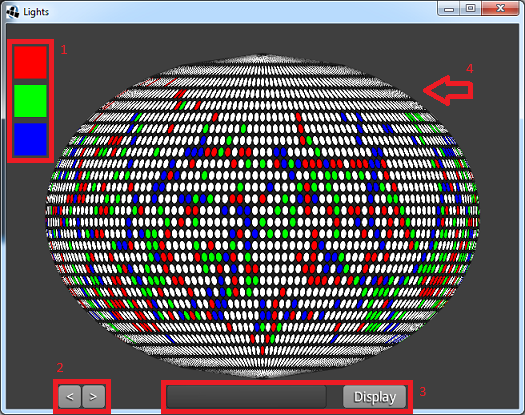
\includegraphics[]{C:/Users/KevinD/Documents/GitHub/blinkylights/doc/user_doc/a_labels.PNG}
\\\\
1. Click on a color to change the color of the brush. The color black is the eraser. Any LEDs colored black will not turn on when the pattern is uploaded to the hardware.
\\\\
2. Click on an arrow to change the rotation of the globe canvas. Left arrow to rotate left. Right arrow to rotate right. Once an arrow is clicked the globe canvas will continuously rotate forever until the 'X' button is pressed. The X button stops the globe canvas from rotating.
\\\\
3. For displaying text on the globe please see the section below.
\\\\
4. Pressing the "clear" button sets all the LED pixels on the current layers to black. It clears all colors from the current layer.
\\\\
5. Pressing the "Upload" button will upload the current pattern on the globe canvas and display it on the hardware.
\\\\
6. This is the globe canvas. A single circle on the globe canvas represent an LED on the hardware with repect to position and time.




















\end{document}